\documentclass{scrartcl}
%\usepackage{aeguill}
\usepackage{tikz}
\usepackage[table,xcdraw]{}
\usepackage{float}
\usepackage{multicol, caption}
\usepackage{dirtree}
% Skapalón frá Hlyni Arnórssyni
% Physics Version 0.2 - 10.Jan 2020
% ---------- Blaðsíðustillingar ---------- 
\usepackage{geometry}

\geometry{
	paper=a4paper, % letterpaper lika til
	top=2.5cm, % Top margin
	bottom=2.5cm, % Bottom margin
	left=2.5cm, % Left margin
	right=2.4cm, % Right margin
	headheight=0.75cm, % Header height
	footskip=1.5cm, % Space from the bottom margin to the baseline of the footer
	headsep=0.75cm, % Space from the top margin to the baseline of the header
	%showframe, % Uncomment to show how the type block is set on the page
}

% ---------- Íslenska ---------- 
\usepackage[T1]{fontenc}
\usepackage[utf8]{inputenc}
% \usepackage[icelandic]{babel}

% ---------- Stærðfræðipakkar frá AMS ---------- 

% \usepackage{amsmath, amsfonts, amsthm, amssymb} % Stærðfræðipakkar

% ---------- Listar/ númeringar ---------- 
\usepackage{enumitem, multicol}

% ---------- Fyrir innsetningu mynda ---------- 
\usepackage{graphicx, float} 
\usepackage{caption}
\newcommand{\source}[1]{\caption*{Source: {#1}} }
\graphicspath{ {./images/} }

%%%%%%%%%%%%%%%%%%%%%%%%%% Hyperlink References %%%%%%%%%%%%%%%%%%%%%%%%%%%
\usepackage[hidelinks, linktoc=all]{hyperref}

%%%%%%%%%%%%%%%%%%%%%%%%% Code blocks %%%%%%%%%%%%%%%%%%%%%%%%%%%%%%%%%%%%%
\usepackage{listings} %code extracts
%\usepackage{xcolor} %custom colours
\usepackage{mdframed} %nice frames
\usepackage{pgffor} % for loops


%% Colors and stuff for plantuml
%%

\setlength\parindent{0pt} % remove need for \noindent
% page numbering
\pagestyle{plain}

%support for figures in multicol environment
\newenvironment{Figure}
  {\par\medskip\noindent\minipage{\linewidth}}
  {\endminipage\par\medskip}

% ---------- Skrá fyrir myndir ---------- 
\graphicspath{{graphics/}{Graphics/}{./}}

\begin{document}

%% --- Titil síða / Title page --- %%
\begin{titlepage}
	\centering
	
\includegraphics[width=0.3\textwidth]{ru-logo.eps}\par\vspace{1cm} %<-- RU Logo
	{\scshape\LARGE Reykjavík University\par} %<-- Nafn háskólans (Háskólinn í Reykjavík / Reykjavik University)
	\vspace{1cm}
	{\scshape\Large Verklegt námskeið II\par} %<-- Áfanga titill / Class or course title
	\vspace{1.5cm}
	{\huge\bfseries Design Report\par} %<-- Titill Skýrslu / Title of Report
	{\Large\itshape  Group 2 \par}
	\vspace{2cm}
	{\Large\itshape Helgi Hákonarson}\par %<-- Nafn nemanda / Name of student
	\texttt{helgihak20@ru.is}\par %<-- t-póstfang / e-mail
	\vspace{0.5cm}
	{\Large\itshape Konráð Elí Sigurgeirsson}\par %<-- Nafn nemanda / Name of student
	\texttt{konrad21@ru.is}\par %<-- t-póstfang / e-mail
	\vspace{0.5cm}
	{\Large\itshape Patrekur Þór Agnarsson}\par %<-- Nafn nemanda / Name of student
	\texttt{patrekur20@ru.is}\par %<-- t-póstfang / e-mail
	\vspace{0.5cm}
	{\Large\itshape Sigurður Baldvin Friðriksson}\par %<-- Nafn nemanda / Name of student
	\texttt{sigurdurf21@ru.is}\par %<-- t-póstfang / e-mail
	\vfill
	Teacher\par %<-- (Umsjón höfðu / supervised by)
	Arnar Leifsson%<-- Nafn kennara og aðstoðarkennara í tilraun / Name of Lab Teacher and TA
	\vfill

% Bottom of the page
	{\large \today\par}
\end{titlepage}

% Efnisyfirlit
\tableofcontents
\newpage

%% --- Titil síða endar / Title page ends --- %%

\section{Introduction}

FireSale! continues to grow and the online marketplace design is becoming more structured. The team behind FireSale! has goals of creating a powerful online presence that creates great opportunities for it's users for online sales and purchases of items of all kinds and sizes. The designs found within this report will become vital building blocks for the coming weeks when programming the front end, back end and database will take place. \\

 The team wanted the appearance of FireSale! to represent it's name so a prototype was created using Figma using a color palette promoting colors of fire. The prototype displays how the user can navigate the website but with no real functionality behind it. This design was also based off wireframes used in the previous phase so a similar navigation for the website is present with minor adjustments being made to fix previous design flaws. \\

 Foundation has been laid for programming with a class diagram being made to identify key objects and attributes of the product. Programming rules have been decided on to maintain nice and clean, readable code that has good form all around. And a navigation diagram to have a good sense of how to connect paths throughout the website. All of this work can be found within this report. \\\\

\section{Prototype}
    The prototype continued our focus around our goal of keeping the site as simple as possible for users. With the useful feedback from our low-fidelity prototype interview we managed to fix some glaring problems whilst making the site even more user friendly. \\
    
    We put emphasis on making the buttons stand out from other non-interactive visual elements and have at most 5 steps for each given action. This was reflected in the exercises we used in the user testing. \\
    
    The following images show most of the functionality for the site with a reasonable flow from picture to picture.\\ 
    An interactive version can be found \href{https://www.figma.com/proto/p44K48Y8N3ytdBPw2n98my/Verk2?node-id=66\%3A183&scaling=min-zoom&page-id=59\%3A72&starting-point-node-id=66\%3A183}{\textcolor{blue}{here}}
     \\
\foreach \n in {1,...,17}{
\begin{Figure}
    \begin{center}
        \includegraphics[width=150mm, height=100mm]{Images/Prototype/prototype\n.png}
\captionof{figure}{Prototype image \n}
    \end{center}
\end{Figure}
}

\section{User Testing}

For our user tests we had an opportunity to do a heuristic evaluation and a general user test, first one with a computer science student who does professional tests for different programs and second round with a student not involved with computer science. Both tests were made on Reykjavík University campus on April 29th 2022 in a private room where users had to solve 9 different tasks with varying difficulty.\\

Overall user testing solidified the teams work on the design and showed an overall average accuracy of 100\% and all tasks were a success, though general speed of tasks was inconsistent between users as expected. Feedback was also positive overall and the users expressed good thoughts of the simplicity of navigating between different pages.\\

We consider the results of user testing a overwhelming success on this design phase and are happy with the result.\\

\subsection{User test objectives}
\begin{itemize}
    \item Register a new user.
    \item Log your user off the website.
    \item Login your user to the website.
    \item Change your bio.
    \item Find a processor using the search engine.
    \item Find a Intel i5 processor under the category electronics.
    \item Put an item up for sale.
    \item Make a bid for a Intel i5 processor.
    \item Accept an offer to a bag that you are selling.
    \item Finish checkout for a intel i5 processor you have bid for.
\end{itemize}

\section{Models, services and views}
In this section we outline our plan for the models, services and views for FireSale!\\

To minimize friction in development, our models are annotated with Django model types and our model classes. To simplify the diagrams we omitted one-to-many and many-to-many relationships in favor of a generic Array structure.\\

With the service models, we tried to capture most of the actions that would be required in the application and we wanted to separate concerns reasonably. \\

The views are also somewhat categorized based on the state of the user but also logically based on what the view should be doing and what actions the user is trying to achieve. 
\subsection{Diagrams}
% generated by Plantuml 1.2022.0       
\definecolor{plantucolor0000}{RGB}{255,255,255}
\definecolor{plantucolor0001}{RGB}{0,0,0}
\definecolor{plantucolor0002}{RGB}{254,254,206}
\definecolor{plantucolor0003}{RGB}{168,0,54}
\definecolor{plantucolor0004}{RGB}{173,209,178}
\definecolor{plantucolor0005}{RGB}{132,190,132}
\definecolor{plantucolor0006}{RGB}{3,128,72}
\definecolor{plantucolor0007}{RGB}{235,147,127}
% Models
\scalebox{0.42}{
\begin{tikzpicture}[yscale=-1
,pstyle1/.style={color=plantucolor0003,fill=plantucolor0002,line width=1.5pt}
,pstyle2/.style={color=plantucolor0003,fill=plantucolor0004,line width=1.0pt}
,pstyle3/.style={color=plantucolor0003,line width=1.5pt}
,pstyle4/.style={color=plantucolor0003,line width=1.0pt}
,pstyle6/.style={color=plantucolor0003,fill=plantucolor0007,line width=1.0pt}
]
\draw[color=black,fill=white,line width=1.5pt] (7pt,7pt) rectangle (1166pt,670pt);
\node at (527.4446pt,9pt)[below right,color=black]{\textbf{FireSale! models}};
\draw[pstyle1] (743.5pt,42pt) rectangle (868.4624pt,153.2446pt);
\draw[pstyle2] (788.4529pt,58pt) ellipse (11pt and 11pt);
\node at (788.4529pt,58pt)[]{\textbf{\Large C}};
\node at (808.9529pt,51.1006pt)[below right,color=black]{User};
\draw[pstyle3] (744.5pt,74pt) -- (867.4624pt,74pt);
\node at (749.5pt,78pt)[below right,color=black]{id: BigAutoField};
\node at (749.5pt,90.6489pt)[below right,color=black]{full\_name: CharField};
\node at (749.5pt,103.2979pt)[below right,color=black]{user\_name: CharField};
\node at (749.5pt,115.9468pt)[below right,color=black]{email: EmailField};
\node at (749.5pt,128.5957pt)[below right,color=black]{password: CharField};
\draw[pstyle3] (744.5pt,145.2446pt) -- (867.4624pt,145.2446pt);
\draw[pstyle1] (982.5pt,384pt) rectangle (1149.3571pt,495.2446pt);
\draw[pstyle2] (1045.0929pt,400pt) ellipse (11pt and 11pt);
\node at (1045.0929pt,400pt)[]{\textbf{\Large C}};
\node at (1065.5929pt,393.1006pt)[below right,color=black]{Order};
\draw[pstyle3] (983.5pt,416pt) -- (1148.3571pt,416pt);
\node at (988.5pt,420pt)[below right,color=black]{id: BigAutoField};
\node at (988.5pt,432.6489pt)[below right,color=black]{buyer: User};
\node at (988.5pt,445.2979pt)[below right,color=black]{seller: User};
\node at (988.5pt,457.9468pt)[below right,color=black]{order\_items: OrderItems};
\draw[pstyle4] (983.5pt,474.5957pt) -- (1148.3571pt,474.5957pt);
\node at (988.5pt,478.5957pt)[below right,color=black]{displayOrderSummary(): void};
\draw[pstyle1] (600pt,396.5pt) rectangle (753.6708pt,482.4468pt);
\draw[pstyle2] (641.0585pt,412.5pt) ellipse (11pt and 11pt);
\node at (641.0585pt,412.5pt)[]{\textbf{\Large C}};
\node at (660.8493pt,405.6006pt)[below right,color=black]{OrderItems};
\draw[pstyle3] (601pt,428.5pt) -- (752.6708pt,428.5pt);
\node at (606pt,432.5pt)[below right,color=black]{order\_id: BigIntergerField};
\node at (606pt,445.1489pt)[below right,color=black]{items: Array\textless Item\textgreater };
\draw[pstyle4] (601pt,461.7979pt) -- (752.6708pt,461.7979pt);
\draw[color=plantucolor0006,fill=plantucolor0005,line width=1.0pt] (611pt,472.7979pt) ellipse (3pt and 3pt);
\node at (620pt,465.7979pt)[below right,color=black]{getTotal(): DecimalField};
\draw[pstyle1] (642.5pt,232pt) rectangle (787.171pt,305.2979pt);
\draw[pstyle2] (674.4013pt,248pt) ellipse (11pt and 11pt);
\node at (674.4013pt,248pt)[]{\textbf{\Large C}};
\node at (692.1572pt,241.1006pt)[below right,color=black]{OrderHistory};
\draw[pstyle3] (643.5pt,264pt) -- (786.171pt,264pt);
\node at (648.5pt,268pt)[below right,color=black]{user\_id: BigIntergerField};
\node at (648.5pt,280.6489pt)[below right,color=black]{orderArray: Array\textless Order\textgreater };
\draw[pstyle3] (643.5pt,297.2979pt) -- (786.171pt,297.2979pt);
\draw[pstyle1] (789pt,384pt) rectangle (947.3091pt,495.2446pt);
\draw[pstyle2] (808.7374pt,400pt) ellipse (11pt and 11pt);
\node at (808.7374pt,400pt)[]{\textbf{\Large C}};
\node at (823.7902pt,393.1006pt)[below right,color=black]{PaymentInformation};
\draw[pstyle3] (790pt,416pt) -- (946.3091pt,416pt);
\node at (795pt,420pt)[below right,color=black]{cardholder\_name: CharField};
\node at (795pt,432.6489pt)[below right,color=black]{card\_number: CharField};
\node at (795pt,445.2979pt)[below right,color=black]{cvc: CharField};
\node at (795pt,457.9468pt)[below right,color=black]{expiry\_month: IntegerField};
\node at (795pt,470.5957pt)[below right,color=black]{expiry\_year: IntergerField};
\draw[pstyle3] (790pt,487.2446pt) -- (946.3091pt,487.2446pt);
\draw[pstyle1] (976.5pt,555pt) rectangle (1149.5266pt,653.5957pt);
\draw[pstyle2] (1014.9877pt,571pt) ellipse (11pt and 11pt);
\node at (1014.9877pt,571pt)[]{\textbf{\Large C}};
\node at (1034.2072pt,564.1006pt)[below right,color=black]{ShippingDetails};
\draw[pstyle3] (977.5pt,587pt) -- (1148.5266pt,587pt);
\node at (982.5pt,591pt)[below right,color=black]{full\_name: CharField};
\node at (982.5pt,603.6489pt)[below right,color=black]{address: CharField};
\node at (982.5pt,616.2979pt)[below right,color=black]{postal\_code: SmallIntegerField};
\node at (982.5pt,628.9468pt)[below right,color=black]{city: CharField};
\draw[pstyle3] (977.5pt,645.5957pt) -- (1148.5266pt,645.5957pt);
\draw[pstyle1] (189.5pt,213pt) rectangle (410.6915pt,324.2446pt);
\draw[pstyle2] (283.2458pt,229pt) ellipse (11pt and 11pt);
\node at (283.2458pt,229pt)[]{\textbf{\Large C}};
\node at (303.7458pt,222.1006pt)[below right,color=black]{Item};
\draw[pstyle3] (190.5pt,245pt) -- (409.6915pt,245pt);
\node at (195.5pt,249pt)[below right,color=black]{id: BigAutoField};
\node at (195.5pt,261.6489pt)[below right,color=black]{price: DecimalField};
\node at (195.5pt,274.2979pt)[below right,color=black]{condition: ConditionType};
\node at (195.5pt,286.9468pt)[below right,color=black]{category: Category};
\node at (195.5pt,299.5957pt)[below right,color=black]{delivery\_Options: Array\textless DeliveryType\textgreater };
\draw[pstyle3] (190.5pt,316.2446pt) -- (409.6915pt,316.2446pt);
\draw[pstyle1] (167.5pt,390pt) rectangle (346.2195pt,488.5957pt);
\draw[pstyle6] (210.5387pt,406pt) ellipse (11pt and 11pt);
\node at (210.5387pt,406pt)[]{\textbf{\Large E}};
\node at (230.7695pt,399.1006pt)[below right,color=black]{ConditionType};
\draw[pstyle3] (168.5pt,422pt) -- (345.2195pt,422pt);
\node at (173.5pt,426pt)[below right,color=black]{NEW};
\node at (173.5pt,438.6489pt)[below right,color=black]{USED};
\node at (173.5pt,451.2979pt)[below right,color=black]{USED\_LIKE\_NEW};
\node at (173.5pt,463.9468pt)[below right,color=black]{FOR\_PARTS\_NOT\_WORKING};
\draw[pstyle3] (168.5pt,480.5957pt) -- (345.2195pt,480.5957pt);
\draw[pstyle1] (904pt,61pt) rectangle (1054.324pt,134.2979pt);
\draw[pstyle2] (936.3993pt,77pt) ellipse (11pt and 11pt);
\node at (936.3993pt,77pt)[]{\textbf{\Large C}};
\node at (954.2658pt,70.1006pt)[below right,color=black]{SearchHistory};
\draw[pstyle3] (905pt,93pt) -- (1053.324pt,93pt);
\node at (910pt,97pt)[below right,color=black]{search\_string: CharField};
\node at (910pt,109.6489pt)[below right,color=black]{timestamp: DateTimeField};
\draw[pstyle3] (905pt,126.2979pt) -- (1053.324pt,126.2979pt);
\draw[pstyle1] (381.5pt,396.5pt) rectangle (564.8677pt,482.4468pt);
\draw[pstyle2] (443.506pt,412.5pt) ellipse (11pt and 11pt);
\node at (443.506pt,412.5pt)[]{\textbf{\Large C}};
\node at (464.006pt,405.6006pt)[below right,color=black]{Category};
\draw[pstyle3] (382.5pt,428.5pt) -- (563.8677pt,428.5pt);
\node at (387.5pt,432.5pt)[below right,color=black]{id: BigAutoField};
\node at (387.5pt,445.1489pt)[below right,color=black]{name: CharField};
\node at (387.5pt,457.7979pt)[below right,color=black]{sub\_categories: Array\textless Category\textgreater };
\draw[pstyle3] (382.5pt,474.4468pt) -- (563.8677pt,474.4468pt);
\draw[pstyle1] (823pt,213pt) rectangle (973.324pt,324.2446pt);
\draw[pstyle2] (868.3342pt,229pt) ellipse (11pt and 11pt);
\node at (868.3342pt,229pt)[]{\textbf{\Large C}};
\node at (888.8342pt,222.1006pt)[below right,color=black]{UserBids};
\draw[pstyle3] (824pt,245pt) -- (972.324pt,245pt);
\node at (829pt,249pt)[below right,color=black]{user\_id: BigIntergerField};
\node at (829pt,261.6489pt)[below right,color=black]{item\_id: BigIntergerField};
\node at (829pt,274.2979pt)[below right,color=black]{amount: BigIntergerField};
\node at (829pt,286.9468pt)[below right,color=black]{timestamp: DateTimeField};
\node at (829pt,299.5957pt)[below right,color=black]{expires: DateTimeField};
\draw[pstyle3] (824pt,316.2446pt) -- (972.324pt,316.2446pt);
\draw[pstyle1] (1008pt,232pt) rectangle (1149.8897pt,305.2979pt);
\draw[pstyle2] (1047.7303pt,248pt) ellipse (11pt and 11pt);
\node at (1047.7303pt,248pt)[]{\textbf{\Large C}};
\node at (1067.226pt,241.1006pt)[below right,color=black]{UserSales};
\draw[pstyle3] (1009pt,264pt) -- (1148.8897pt,264pt);
\node at (1014pt,268pt)[below right,color=black]{user\_id: BigIntergerField};
\node at (1014pt,280.6489pt)[below right,color=black]{items: Array\textless Item\textgreater };
\draw[pstyle3] (1009pt,297.2979pt) -- (1148.8897pt,297.2979pt);
\draw[pstyle1] (488.5pt,219pt) rectangle (607.2149pt,317.5957pt);
\draw[pstyle2] (512.0041pt,235pt) ellipse (11pt and 11pt);
\node at (512.0041pt,235pt)[]{\textbf{\Large C}};
\node at (527.8939pt,228.1006pt)[below right,color=black]{UserRatings};
\draw[pstyle3] (489.5pt,251pt) -- (606.2149pt,251pt);
\node at (494.5pt,255pt)[below right,color=black]{rater: User};
\node at (494.5pt,267.6489pt)[below right,color=black]{ratee: User};
\node at (494.5pt,280.2979pt)[below right,color=black]{order: Order};
\node at (494.5pt,292.9468pt)[below right,color=black]{rating: DecimalField};
\draw[pstyle3] (489.5pt,309.5957pt) -- (606.2149pt,309.5957pt);
\draw[pstyle1] (595.5pt,61pt) rectangle (708.0079pt,134.2979pt);
\draw[pstyle2] (616.0913pt,77pt) ellipse (11pt and 11pt);
\node at (616.0913pt,77pt)[]{\textbf{\Large C}};
\node at (631.3338pt,70.1006pt)[below right,color=black]{Notfications};
\draw[pstyle3] (596.5pt,93pt) -- (707.0079pt,93pt);
\node at (601.5pt,97pt)[below right,color=black]{id: BigAutoField};
\node at (601.5pt,109.6489pt)[below right,color=black]{message: CharField};
\draw[pstyle3] (596.5pt,126.2979pt) -- (707.0079pt,126.2979pt);
\draw[pstyle1] (23.5pt,396.5pt) rectangle (132.8231pt,482.4468pt);
\draw[pstyle6] (38.5pt,412.5pt) ellipse (11pt and 11pt);
\node at (38.5pt,412.5pt)[]{\textbf{\Large E}};
\node at (52.5pt,405.6006pt)[below right,color=black]{DeliveryType};
\draw[pstyle3] (24.5pt,428.5pt) -- (131.8231pt,428.5pt);
\node at (29.5pt,432.5pt)[below right,color=black]{DELIVERY};
\node at (29.5pt,445.1489pt)[below right,color=black]{PICKUP};
\node at (29.5pt,457.7979pt)[below right,color=black]{HANDOFF};
\draw[pstyle3] (24.5pt,474.4468pt) -- (131.8231pt,474.4468pt);
\draw[pstyle4] (776.45pt,153.37pt) ..controls (762.6pt,179.1pt) and (746.48pt,209.03pt) .. (734.23pt,231.79pt);
\draw[pstyle4] (868.51pt,97.5pt) ..controls (880.31pt,97.5pt) and (892.1pt,97.5pt) .. (903.9pt,97.5pt);
\draw[pstyle4] (770.93pt,305.12pt) ..controls (782.33pt,311.77pt) and (794.39pt,318.39pt) .. (806pt,324pt) ..controls (874pt,356.87pt) and (896.28pt,352.66pt) .. (965pt,384pt) ..controls (970.71pt,386.6pt) and (976.55pt,389.39pt) .. (982.39pt,392.28pt);
\draw[pstyle4] (1003.93pt,383.78pt) ..controls (986.8pt,371.6pt) and (967.42pt,360.43pt) .. (947.5pt,354pt) ..controls (880.68pt,332.41pt) and (856.05pt,331.58pt) .. (789.5pt,354pt) ..controls (763.81pt,362.65pt) and (739.34pt,379.77pt) .. (719.82pt,396.42pt);
\draw[pstyle4] (410.65pt,310.43pt) ..controls (463.28pt,330.91pt) and (526.66pt,357.04pt) .. (582pt,384pt) ..controls (589.86pt,387.83pt) and (597.97pt,392.04pt) .. (605.97pt,396.38pt);
\draw[pstyle4] (835.87pt,153.37pt) ..controls (846.26pt,172.45pt) and (857.9pt,193.84pt) .. (868.28pt,212.91pt);
\draw[pstyle4] (868.51pt,141.18pt) ..controls (874.72pt,145.23pt) and (880.96pt,149.23pt) .. (887pt,153pt) ..controls (932.28pt,181.24pt) and (945.2pt,185.61pt) .. (991pt,213pt) ..controls (1001.03pt,218.99pt) and (1011.63pt,225.46pt) .. (1021.88pt,231.77pt);
\draw[pstyle4] (743.36pt,141.71pt) ..controls (737.52pt,145.58pt) and (731.67pt,149.39pt) .. (726pt,153pt) ..controls (681.96pt,181.04pt) and (668.79pt,184.56pt) .. (625pt,213pt) ..controls (619.37pt,216.66pt) and (613.57pt,220.54pt) .. (607.79pt,224.49pt);
\draw[pstyle4] (286.04pt,324.37pt) ..controls (280.67pt,345.48pt) and (274.58pt,369.41pt) .. (269.37pt,389.89pt);
\draw[pstyle4] (356.17pt,324.37pt) ..controls (380.14pt,347.79pt) and (407.68pt,374.69pt) .. (429.99pt,396.49pt);
\draw[pstyle4] (228.23pt,324.14pt) ..controls (197.19pt,347.76pt) and (161.46pt,374.97pt) .. (132.63pt,396.91pt);
\draw[pstyle4] (947.28pt,439.5pt) ..controls (958.87pt,439.5pt) and (970.47pt,439.5pt) .. (982.06pt,439.5pt);
\draw[pstyle4] (1064.99pt,495.23pt) ..controls (1064.64pt,514.56pt) and (1064.24pt,536.15pt) .. (1063.89pt,554.93pt);
\draw[pstyle4] (708.55pt,97.5pt) ..controls (720.09pt,97.5pt) and (731.64pt,97.5pt) .. (743.19pt,97.5pt);
\end{tikzpicture}
}

\begin{multicols}{2}
% Services
\scalebox{0.48}{
\begin{tikzpicture}[yscale=-1
,pstyle1/.style={color=plantucolor0003,fill=plantucolor0002,line width=1.5pt}
,pstyle2/.style={color=plantucolor0003,fill=plantucolor0004,line width=1.0pt}
,pstyle3/.style={color=plantucolor0003,line width=1.5pt}
,pstyle4/.style={color=plantucolor0006,fill=plantucolor0005,line width=1.0pt}
]
\draw[color=black,fill=white,line width=1.5pt] (7pt,7pt) rectangle (463pt,474pt);
\node at (172.2019pt,9pt)[below right,color=black]{\textbf{FireSale! Services}};
\draw[pstyle1] (26pt,42pt) rectangle (147.9442pt,165.8936pt);
\draw[pstyle2] (51.5242pt,58pt) ellipse (11pt and 11pt);
\node at (51.5242pt,58pt)[]{\textbf{\Large C}};
\node at (67.8629pt,51.1006pt)[below right,color=black]{ItemService};
\draw[pstyle3] (27pt,74pt) -- (146.9442pt,74pt);
\draw[pstyle3] (27pt,82pt) -- (146.9442pt,82pt);
\draw[pstyle4] (37pt,93pt) ellipse (3pt and 3pt);
\node at (46pt,86pt)[below right,color=black]{create\_item()};
\draw[pstyle4] (37pt,105.6489pt) ellipse (3pt and 3pt);
\node at (46pt,98.6489pt)[below right,color=black]{delete\_item()};
\draw[pstyle4] (37pt,118.2979pt) ellipse (3pt and 3pt);
\node at (46pt,111.2979pt)[below right,color=black]{update\_item()};
\draw[pstyle4] (37pt,130.9468pt) ellipse (3pt and 3pt);
\node at (46pt,123.9468pt)[below right,color=black]{get\_all\_items()};
\draw[pstyle4] (37pt,143.5957pt) ellipse (3pt and 3pt);
\node at (46pt,136.5957pt)[below right,color=black]{get\_item\_images()};
\draw[pstyle4] (37pt,156.2446pt) ellipse (3pt and 3pt);
\node at (46pt,149.2446pt)[below right,color=black]{sort\_items()};
\draw[pstyle1] (183.5pt,61pt) rectangle (276.3615pt,146.9468pt);
\draw[pstyle2] (198.5pt,77pt) ellipse (11pt and 11pt);
\node at (198.5pt,77pt)[]{\textbf{\Large C}};
\node at (212.5pt,70.1006pt)[below right,color=black]{BidService};
\draw[pstyle3] (184.5pt,93pt) -- (275.3615pt,93pt);
\draw[pstyle3] (184.5pt,101pt) -- (275.3615pt,101pt);
\draw[pstyle4] (194.5pt,112pt) ellipse (3pt and 3pt);
\node at (203.5pt,105pt)[below right,color=black]{add\_bid()};
\draw[pstyle4] (194.5pt,124.6489pt) ellipse (3pt and 3pt);
\node at (203.5pt,117.6489pt)[below right,color=black]{retract\_bid()};
\draw[pstyle4] (194.5pt,137.2979pt) ellipse (3pt and 3pt);
\node at (203.5pt,130.2979pt)[below right,color=black]{accept\_bid()};
\draw[pstyle1] (312pt,61pt) rectangle (436.1641pt,146.9468pt);
\draw[pstyle2] (327pt,77pt) ellipse (11pt and 11pt);
\node at (327pt,77pt)[]{\textbf{\Large C}};
\node at (341pt,70.1006pt)[below right,color=black]{CategoryService};
\draw[pstyle3] (313pt,93pt) -- (435.1641pt,93pt);
\draw[pstyle3] (313pt,101pt) -- (435.1641pt,101pt);
\draw[pstyle4] (323pt,112pt) ellipse (3pt and 3pt);
\node at (332pt,105pt)[below right,color=black]{create\_category()};
\draw[pstyle4] (323pt,124.6489pt) ellipse (3pt and 3pt);
\node at (332pt,117.6489pt)[below right,color=black]{delete\_category()};
\draw[pstyle4] (323pt,137.2979pt) ellipse (3pt and 3pt);
\node at (332pt,130.2979pt)[below right,color=black]{update\_category()};
\draw[pstyle1] (23.5pt,226pt) rectangle (150.1286pt,324.5957pt);
\draw[pstyle2] (47.5771pt,242pt) ellipse (11pt and 11pt);
\node at (47.5771pt,242pt)[]{\textbf{\Large C}};
\node at (63.5943pt,235.1006pt)[below right,color=black]{OrderService};
\draw[pstyle3] (24.5pt,258pt) -- (149.1286pt,258pt);
\draw[pstyle3] (24.5pt,266pt) -- (149.1286pt,266pt);
\draw[pstyle4] (34.5pt,277pt) ellipse (3pt and 3pt);
\node at (43.5pt,270pt)[below right,color=black]{set\_shipping\_info()};
\draw[pstyle4] (34.5pt,289.6489pt) ellipse (3pt and 3pt);
\node at (43.5pt,282.6489pt)[below right,color=black]{set\_payment\_info()};
\draw[pstyle4] (34.5pt,302.2979pt) ellipse (3pt and 3pt);
\node at (43.5pt,295.2979pt)[below right,color=black]{create\_invoice()};
\draw[pstyle4] (34.5pt,314.9468pt) ellipse (3pt and 3pt);
\node at (43.5pt,307.9468pt)[below right,color=black]{get\_order\_details()};
\draw[pstyle1] (186pt,226pt) rectangle (289.7333pt,324.5957pt);
\draw[pstyle2] (202.7979pt,242pt) ellipse (11pt and 11pt);
\node at (202.7979pt,242pt)[]{\textbf{\Large C}};
\node at (217.1975pt,235.1006pt)[below right,color=black]{UserService};
\draw[pstyle3] (187pt,258pt) -- (288.7333pt,258pt);
\draw[pstyle3] (187pt,266pt) -- (288.7333pt,266pt);
\draw[pstyle4] (197pt,277pt) ellipse (3pt and 3pt);
\node at (206pt,270pt)[below right,color=black]{get\_user\_info()};
\draw[pstyle4] (197pt,289.6489pt) ellipse (3pt and 3pt);
\node at (206pt,282.6489pt)[below right,color=black]{set\_user\_info()};
\draw[pstyle4] (197pt,302.2979pt) ellipse (3pt and 3pt);
\node at (206pt,295.2979pt)[below right,color=black]{delete\_user()};
\draw[pstyle4] (197pt,314.9468pt) ellipse (3pt and 3pt);
\node at (206pt,307.9468pt)[below right,color=black]{create\_user()};
\draw[pstyle1] (325.5pt,239pt) rectangle (446.3267pt,312.2979pt);
\draw[pstyle2] (340.5pt,255pt) ellipse (11pt and 11pt);
\node at (340.5pt,255pt)[]{\textbf{\Large C}};
\node at (354.5pt,248.1006pt)[below right,color=black]{SearchService()};
\draw[pstyle3] (326.5pt,271pt) -- (445.3267pt,271pt);
\draw[pstyle3] (326.5pt,279pt) -- (445.3267pt,279pt);
\draw[pstyle4] (336.5pt,290pt) ellipse (3pt and 3pt);
\node at (345.5pt,283pt)[below right,color=black]{item\_search()};
\draw[pstyle4] (336.5pt,302.6489pt) ellipse (3pt and 3pt);
\node at (345.5pt,295.6489pt)[below right,color=black]{category\_search()};
\draw[pstyle1] (23pt,385pt) rectangle (177.0581pt,458.2979pt);
\draw[pstyle2] (40.0843pt,401pt) ellipse (11pt and 11pt);
\node at (40.0843pt,401pt)[]{\textbf{\Large C}};
\node at (54.5475pt,394.1006pt)[below right,color=black]{NotificationService()};
\draw[pstyle3] (24pt,417pt) -- (176.0581pt,417pt);
\draw[pstyle3] (24pt,425pt) -- (176.0581pt,425pt);
\draw[pstyle4] (34pt,436pt) ellipse (3pt and 3pt);
\node at (43pt,429pt)[below right,color=black]{send\_notification()};
\draw[pstyle4] (34pt,448.6489pt) ellipse (3pt and 3pt);
\node at (43pt,441.6489pt)[below right,color=black]{mark\_notification\_read()};
\draw[pstyle1] (212pt,391pt) rectangle (333.8316pt,451.6489pt);
\draw[pstyle2] (227pt,407pt) ellipse (11pt and 11pt);
\node at (227pt,407pt)[]{\textbf{\Large C}};
\node at (241pt,400.1006pt)[below right,color=black]{PaymentService};
\draw[pstyle3] (213pt,423pt) -- (332.8316pt,423pt);
\draw[pstyle3] (213pt,431pt) -- (332.8316pt,431pt);
\draw[pstyle4] (223pt,442pt) ellipse (3pt and 3pt);
\node at (232pt,435pt)[below right,color=black]{verify\_payment()};
\end{tikzpicture}
}

% Views
\scalebox{0.595}{
\begin{tikzpicture}[yscale=-1
,pstyle1/.style={color=plantucolor0003,fill=plantucolor0002,line width=1.5pt}
,pstyle2/.style={color=plantucolor0003,fill=plantucolor0004,line width=1.0pt}
,pstyle3/.style={color=plantucolor0003,line width=1.5pt}
,pstyle4/.style={color=plantucolor0006,fill=plantucolor0005,line width=1.0pt}
]
\draw[color=black,fill=white,line width=1.5pt] (7pt,7pt) rectangle (314pt,341pt);
\node at (105.8872pt,9pt)[below right,color=black]{\textbf{FireSale! Views}};
\draw[pstyle1] (23.5pt,67.5pt) rectangle (134.5118pt,140.7979pt);
\draw[pstyle2] (38.5pt,83.5pt) ellipse (11pt and 11pt);
\node at (38.5pt,83.5pt)[]{\textbf{\Large C}};
\node at (52.5pt,76.6006pt)[below right,color=black]{GeneralViews};
\draw[pstyle3] (24.5pt,99.5pt) -- (133.5118pt,99.5pt);
\draw[pstyle3] (24.5pt,107.5pt) -- (133.5118pt,107.5pt);
\draw[pstyle4] (34.5pt,118.5pt) ellipse (3pt and 3pt);
\node at (43.5pt,111.5pt)[below right,color=black]{home()};
\draw[pstyle4] (34.5pt,131.1489pt) ellipse (3pt and 3pt);
\node at (43.5pt,124.1489pt)[below right,color=black]{search\_results()};
\draw[pstyle1] (170pt,42pt) rectangle (264.0129pt,165.8936pt);
\draw[pstyle2] (185.0791pt,58pt) ellipse (11pt and 11pt);
\node at (185.0791pt,58pt)[]{\textbf{\Large C}};
\node at (199.0967pt,51.1006pt)[below right,color=black]{UserViews};
\draw[pstyle3] (171pt,74pt) -- (263.0129pt,74pt);
\draw[pstyle3] (171pt,82pt) -- (263.0129pt,82pt);
\draw[pstyle4] (181pt,93pt) ellipse (3pt and 3pt);
\node at (190pt,86pt)[below right,color=black]{login()};
\draw[pstyle4] (181pt,105.6489pt) ellipse (3pt and 3pt);
\node at (190pt,98.6489pt)[below right,color=black]{logout()};
\draw[pstyle4] (181pt,118.2979pt) ellipse (3pt and 3pt);
\node at (190pt,111.2979pt)[below right,color=black]{profile()};
\draw[pstyle4] (181pt,130.9468pt) ellipse (3pt and 3pt);
\node at (190pt,123.9468pt)[below right,color=black]{active\_bids()};
\draw[pstyle4] (181pt,143.5957pt) ellipse (3pt and 3pt);
\node at (190pt,136.5957pt)[below right,color=black]{active\_sales()};
\draw[pstyle4] (181pt,156.2446pt) ellipse (3pt and 3pt);
\node at (190pt,149.2446pt)[below right,color=black]{notification()};
\draw[pstyle1] (23.5pt,239pt) rectangle (116.0538pt,312.2979pt);
\draw[pstyle2] (38.5pt,255pt) ellipse (11pt and 11pt);
\node at (38.5pt,255pt)[]{\textbf{\Large C}};
\node at (52.5pt,248.1006pt)[below right,color=black]{ItemViews};
\draw[pstyle3] (24.5pt,271pt) -- (115.0538pt,271pt);
\draw[pstyle3] (24.5pt,279pt) -- (115.0538pt,279pt);
\draw[pstyle4] (34.5pt,290pt) ellipse (3pt and 3pt);
\node at (43.5pt,283pt)[below right,color=black]{item\_page()};
\draw[pstyle4] (34.5pt,302.6489pt) ellipse (3pt and 3pt);
\node at (43.5pt,295.6489pt)[below right,color=black]{item\_bid()};
\draw[pstyle1] (152pt,226pt) rectangle (298.1945pt,324.5957pt);
\draw[pstyle2] (178.6738pt,242pt) ellipse (11pt and 11pt);
\node at (178.6738pt,242pt)[]{\textbf{\Large C}};
\node at (195.268pt,235.1006pt)[below right,color=black]{CheckoutViews};
\draw[pstyle3] (153pt,258pt) -- (297.1945pt,258pt);
\draw[pstyle3] (153pt,266pt) -- (297.1945pt,266pt);
\draw[pstyle4] (163pt,277pt) ellipse (3pt and 3pt);
\node at (172pt,270pt)[below right,color=black]{customer\_info()};
\draw[pstyle4] (163pt,289.6489pt) ellipse (3pt and 3pt);
\node at (172pt,282.6489pt)[below right,color=black]{delivery\_method()};
\draw[pstyle4] (163pt,302.2979pt) ellipse (3pt and 3pt);
\node at (172pt,295.2979pt)[below right,color=black]{payment\_information()};
\draw[pstyle4] (163pt,314.9468pt) ellipse (3pt and 3pt);
\node at (172pt,307.9468pt)[below right,color=black]{order\_confirmed()};
\end{tikzpicture}
}
\end{multicols}

\section{State diagram}



% generated by Plantuml 1.2022.0       
\definecolor{plantucolor0000}{RGB}{254,254,206}
\definecolor{plantucolor0001}{RGB}{168,0,54}
\definecolor{plantucolor0002}{RGB}{255,255,255}
\definecolor{plantucolor0003}{RGB}{0,0,0}
\begin{tikzpicture}[yscale=-1
,pstyle0/.style={color=plantucolor0001,fill=plantucolor0000,line width=1.5pt}
,pstyle2/.style={color=plantucolor0001,line width=1.5pt}
,pstyle3/.style={fill=black,line width=1.0pt}
,pstyle5/.style={color=plantucolor0001,line width=1.0pt}
,pstyle6/.style={color=plantucolor0001,fill=plantucolor0001,line width=1.0pt}
]
\draw[pstyle0] (7pt,32pt) arc (180:270:25pt) -- (32pt,7pt) -- (275.4835pt,7pt) arc (270:360:25pt) -- (300.4835pt,32pt) -- (300.4835pt,286.7999pt) arc (0:90:25pt) -- (275.4835pt,311.7999pt) -- (32pt,311.7999pt) arc (90:180:25pt) -- (7pt,286.7999pt) -- cycle;
\draw[color=white,fill=white,line width=1.0pt] (10pt,61.7999pt) arc (180:270:25pt) -- (35pt,36.7999pt) -- (272.4835pt,36.7999pt) arc (270:360:25pt) -- (297.4835pt,61.7999pt) -- (297.4835pt,283.7999pt) arc (0:90:25pt) -- (272.4835pt,308.7999pt) -- (35pt,308.7999pt) arc (90:180:25pt) -- (10pt,283.7999pt) -- cycle;
\draw[pstyle2] (7pt,33.7999pt) -- (300.4835pt,33.7999pt);
\node at (141.7417pt,12pt)[below right,color=black]{Bid};
\draw[pstyle0] (99pt,65.7999pt) arc (180:270:20pt) -- (119pt,45.7999pt) -- (147.08pt,45.7999pt) arc (270:360:20pt) -- (167.08pt,65.7999pt) -- (167.08pt,65.7999pt) arc (0:90:20pt) -- (147.08pt,85.7999pt) -- (119pt,85.7999pt) arc (90:180:20pt) -- (99pt,65.7999pt) -- cycle;
\node at (104pt,57.4pt)[below right,color=black]{New Bid};
\draw[pstyle0] (110pt,197.7999pt) arc (180:270:25pt) -- (135pt,172.7999pt) -- (233.4pt,172.7999pt) arc (270:360:25pt) -- (258.4pt,197.7999pt) -- (258.4pt,213.4001pt) arc (0:90:25pt) -- (233.4pt,238.4001pt) -- (135pt,238.4001pt) arc (90:180:25pt) -- (110pt,213.4001pt) -- cycle;
\draw[pstyle2] (110pt,199.5999pt) -- (258.4pt,199.5999pt);
\node at (138.0152pt,177.7999pt)[below right,color=black]{New Max Bid};
\node at (115pt,204.5999pt)[below right,color=black]{do / notify seller};
\node at (115pt,219pt)[below right,color=black]{do / update max bid};
\draw[pstyle0] (19pt,128.7999pt) arc (180:270:25pt) -- (44pt,103.7999pt) -- (125.6pt,103.7999pt) arc (270:360:25pt) -- (150.6pt,128.7999pt) -- (150.6pt,130pt) arc (0:90:25pt) -- (125.6pt,155pt) -- (44pt,155pt) arc (90:180:25pt) -- (19pt,130pt) -- cycle;
\draw[pstyle2] (19pt,130.5999pt) -- (150.6pt,130.5999pt);
\node at (45.406pt,108.7999pt)[below right,color=black]{Bid too low};
\node at (24pt,135.5999pt)[below right,color=black]{do / notify buyer};
\draw[pstyle3] (71pt,65.7999pt) ellipse (10pt and 10pt);
\draw[color=black,line width=1.0pt] (94pt,285.7999pt) ellipse (10pt and 10pt);
\draw[pstyle3] (94.5pt,286.2999pt) ellipse (6pt and 6pt);
\draw[pstyle5] (81.17pt,65.7999pt) ..controls (85.44pt,65.7999pt) and (89.71pt,65.7999pt) .. (93.98pt,65.7999pt);
\draw[pstyle6] (98.99pt,65.7999pt) -- (89.99pt,61.7999pt) -- (93.99pt,65.7999pt) -- (89.99pt,69.7999pt) -- (98.99pt,65.7999pt) -- cycle;
\draw[pstyle5] (147.81pt,86.0399pt) ..controls (151.54pt,91.5499pt) and (155.26pt,97.7199pt) .. (158pt,103.7999pt) ..controls (167.04pt,123.8699pt) and (173.35pt,147.6599pt) .. (177.5pt,167.0999pt);
\draw[pstyle6] (178.61pt,172.4599pt) -- (180.7027pt,162.836pt) -- (177.5965pt,167.5637pt) -- (172.8687pt,164.4576pt) -- (178.61pt,172.4599pt) -- cycle;
\node at (175pt,121.7999pt)[below right,color=black]{[new bid \textgreater  old bid]};
\draw[pstyle5] (118.08pt,85.9199pt) ..controls (114.7pt,90.2399pt) and (111.05pt,94.9199pt) .. (107.45pt,99.5399pt);
\draw[pstyle6] (104.16pt,103.7499pt) -- (112.8568pt,99.1276pt) -- (107.2415pt,99.8124pt) -- (106.5568pt,94.1971pt) -- (104.16pt,103.7499pt) -- cycle;
\draw[pstyle5] (86.45pt,155.1199pt) ..controls (88.35pt,187.7699pt) and (91.63pt,244.0799pt) .. (93.16pt,270.4299pt);
\draw[pstyle6] (93.46pt,275.5699pt) -- (96.9138pt,266.3465pt) -- (93.1605pt,270.5789pt) -- (88.9282pt,266.8257pt) -- (93.46pt,275.5699pt) -- cycle;
\draw[pstyle5] (146.87pt,238.9799pt) ..controls (131.83pt,252.0199pt) and (115.57pt,266.1099pt) .. (105.11pt,275.1699pt);
\draw[pstyle6] (101.27pt,278.4999pt) -- (110.695pt,275.6419pt) -- (105.0532pt,275.2307pt) -- (105.4643pt,269.5888pt) -- (101.27pt,278.4999pt) -- cycle;
\end{tikzpicture}\\\\

% generated by Plantuml 1.2022.0       
\definecolor{plantucolor0000}{RGB}{254,254,206}
\definecolor{plantucolor0001}{RGB}{168,0,54}
\definecolor{plantucolor0002}{RGB}{255,255,255}
\definecolor{plantucolor0003}{RGB}{0,0,0}
\begin{tikzpicture}[yscale=-1
,pstyle0/.style={color=plantucolor0001,fill=plantucolor0000,line width=1.5pt}
,pstyle2/.style={color=plantucolor0001,line width=1.5pt}
,pstyle3/.style={fill=black,line width=1.0pt}
,pstyle5/.style={color=plantucolor0001,line width=1.0pt}
,pstyle6/.style={color=plantucolor0001,fill=plantucolor0001,line width=1.0pt}
]
\draw[pstyle0] (7pt,32pt) arc (180:270:25pt) -- (32pt,7pt) -- (360.4923pt,7pt) arc (270:360:25pt) -- (385.4923pt,32pt) -- (385.4923pt,300.7999pt) arc (0:90:25pt) -- (360.4923pt,325.7999pt) -- (32pt,325.7999pt) arc (90:180:25pt) -- (7pt,300.7999pt) -- cycle;
\draw[color=white,fill=white,line width=1.0pt] (10pt,61.7999pt) arc (180:270:25pt) -- (35pt,36.7999pt) -- (357.4923pt,36.7999pt) arc (270:360:25pt) -- (382.4923pt,61.7999pt) -- (382.4923pt,297.7999pt) arc (0:90:25pt) -- (357.4923pt,322.7999pt) -- (35pt,322.7999pt) arc (90:180:25pt) -- (10pt,297.7999pt) -- cycle;
\draw[pstyle2] (7pt,33.7999pt) -- (385.4923pt,33.7999pt);
\node at (129.5789pt,12pt)[below right,color=black]{Accept / decline bid};
\draw[pstyle0] (19pt,212.7999pt) arc (180:270:25pt) -- (44pt,187.7999pt) -- (184.2573pt,187.7999pt) arc (270:360:25pt) -- (209.2573pt,212.7999pt) -- (209.2573pt,228.4001pt) arc (0:90:25pt) -- (184.2573pt,253.4001pt) -- (44pt,253.4001pt) arc (90:180:25pt) -- (19pt,228.4001pt) -- cycle;
\draw[pstyle2] (19pt,214.5999pt) -- (209.2573pt,214.5999pt);
\node at (71.7822pt,192.7999pt)[below right,color=black]{Bid declined};
\node at (24pt,219.5999pt)[below right,color=black]{do / notify bidder};
\node at (24pt,234pt)[below right,color=black]{do / find second highest bid};
\draw[pstyle0] (210.5pt,125.7999pt) arc (180:270:25pt) -- (235.5pt,100.7999pt) -- (314.7pt,100.7999pt) arc (270:360:25pt) -- (339.7pt,125.7999pt) -- (339.7pt,127pt) arc (0:90:25pt) -- (314.7pt,152pt) -- (235.5pt,152pt) arc (90:180:25pt) -- (210.5pt,127pt) -- cycle;
\draw[pstyle2] (210.5pt,127.5999pt) -- (339.7pt,127.5999pt);
\node at (232.1778pt,105.7999pt)[below right,color=black]{Bid accepted};
\node at (215.5pt,132.5999pt)[below right,color=black]{do / notify buyer};
\draw[pstyle0] (227pt,220.7999pt) arc (180:270:25pt) -- (252pt,195.7999pt) -- (344.4923pt,195.7999pt) arc (270:360:25pt) -- (369.4923pt,220.7999pt) -- (369.4923pt,220.7999pt) arc (0:90:25pt) -- (344.4923pt,245.7999pt) -- (252pt,245.7999pt) arc (90:180:25pt) -- (227pt,220.7999pt) -- cycle;
\draw[pstyle2] (227pt,222.5999pt) -- (369.4923pt,222.5999pt);
\node at (237pt,200.7999pt)[below right,color=black]{Awaiting payment};
\draw[pstyle3] (205pt,54.7999pt) ellipse (10pt and 10pt);
\draw[color=black,line width=1.0pt] (206pt,299.7999pt) ellipse (10pt and 10pt);
\draw[pstyle3] (206.5pt,300.2999pt) ellipse (6pt and 6pt);
\draw[pstyle5] (200.36pt,64.1599pt) ..controls (188.39pt,85.7399pt) and (155.88pt,144.3299pt) .. (134.34pt,183.1499pt);
\draw[pstyle6] (131.77pt,187.7799pt) -- (139.6226pt,181.8354pt) -- (134.1873pt,183.4031pt) -- (132.6196pt,177.9678pt) -- (131.77pt,187.7799pt) -- cycle;
\draw[pstyle5] (211.71pt,62.4599pt) ..controls (219.78pt,70.4799pt) and (233.84pt,84.4399pt) .. (246.67pt,97.1699pt);
\draw[pstyle6] (250.25pt,100.7199pt) -- (246.6959pt,91.5347pt) -- (246.7073pt,97.1915pt) -- (241.0505pt,97.203pt) -- (250.25pt,100.7199pt) -- cycle;
\draw[pstyle5] (152.48pt,254.0099pt) ..controls (167.78pt,266.8199pt) and (184.23pt,280.5799pt) .. (194.79pt,289.4199pt);
\draw[pstyle6] (198.67pt,292.6599pt) -- (194.3297pt,283.819pt) -- (194.8336pt,289.4534pt) -- (189.1992pt,289.9573pt) -- (198.67pt,292.6599pt) -- cycle;
\draw[pstyle5] (281.16pt,152.0899pt) ..controls (284.1pt,163.8899pt) and (287.63pt,178.0799pt) .. (290.7pt,190.4199pt);
\draw[pstyle6] (291.98pt,195.5799pt) -- (293.7046pt,185.8832pt) -- (290.7808pt,190.7259pt) -- (285.9381pt,187.802pt) -- (291.98pt,195.5799pt) -- cycle;
\draw[pstyle5] (269.14pt,245.9499pt) ..controls (251.53pt,260.6899pt) and (230.01pt,278.7099pt) .. (217.18pt,289.4399pt);
\draw[pstyle6] (213.18pt,292.7899pt) -- (222.6508pt,290.0873pt) -- (217.0164pt,289.5834pt) -- (217.5203pt,283.949pt) -- (213.18pt,292.7899pt) -- cycle;
\end{tikzpicture}


\section{Navigation Diagram}

Our navigation diagram shows in a direct way how different paths can be taken to achieve different results. It covers all of the functions our website provides and will play a vital role moving forward to support our team in programming the website.\\

Having a clear way of moving around a website is a vital part in providing a good solution for users so they can spend more time doing practical work and less time spent on figuring out how to do things.\\

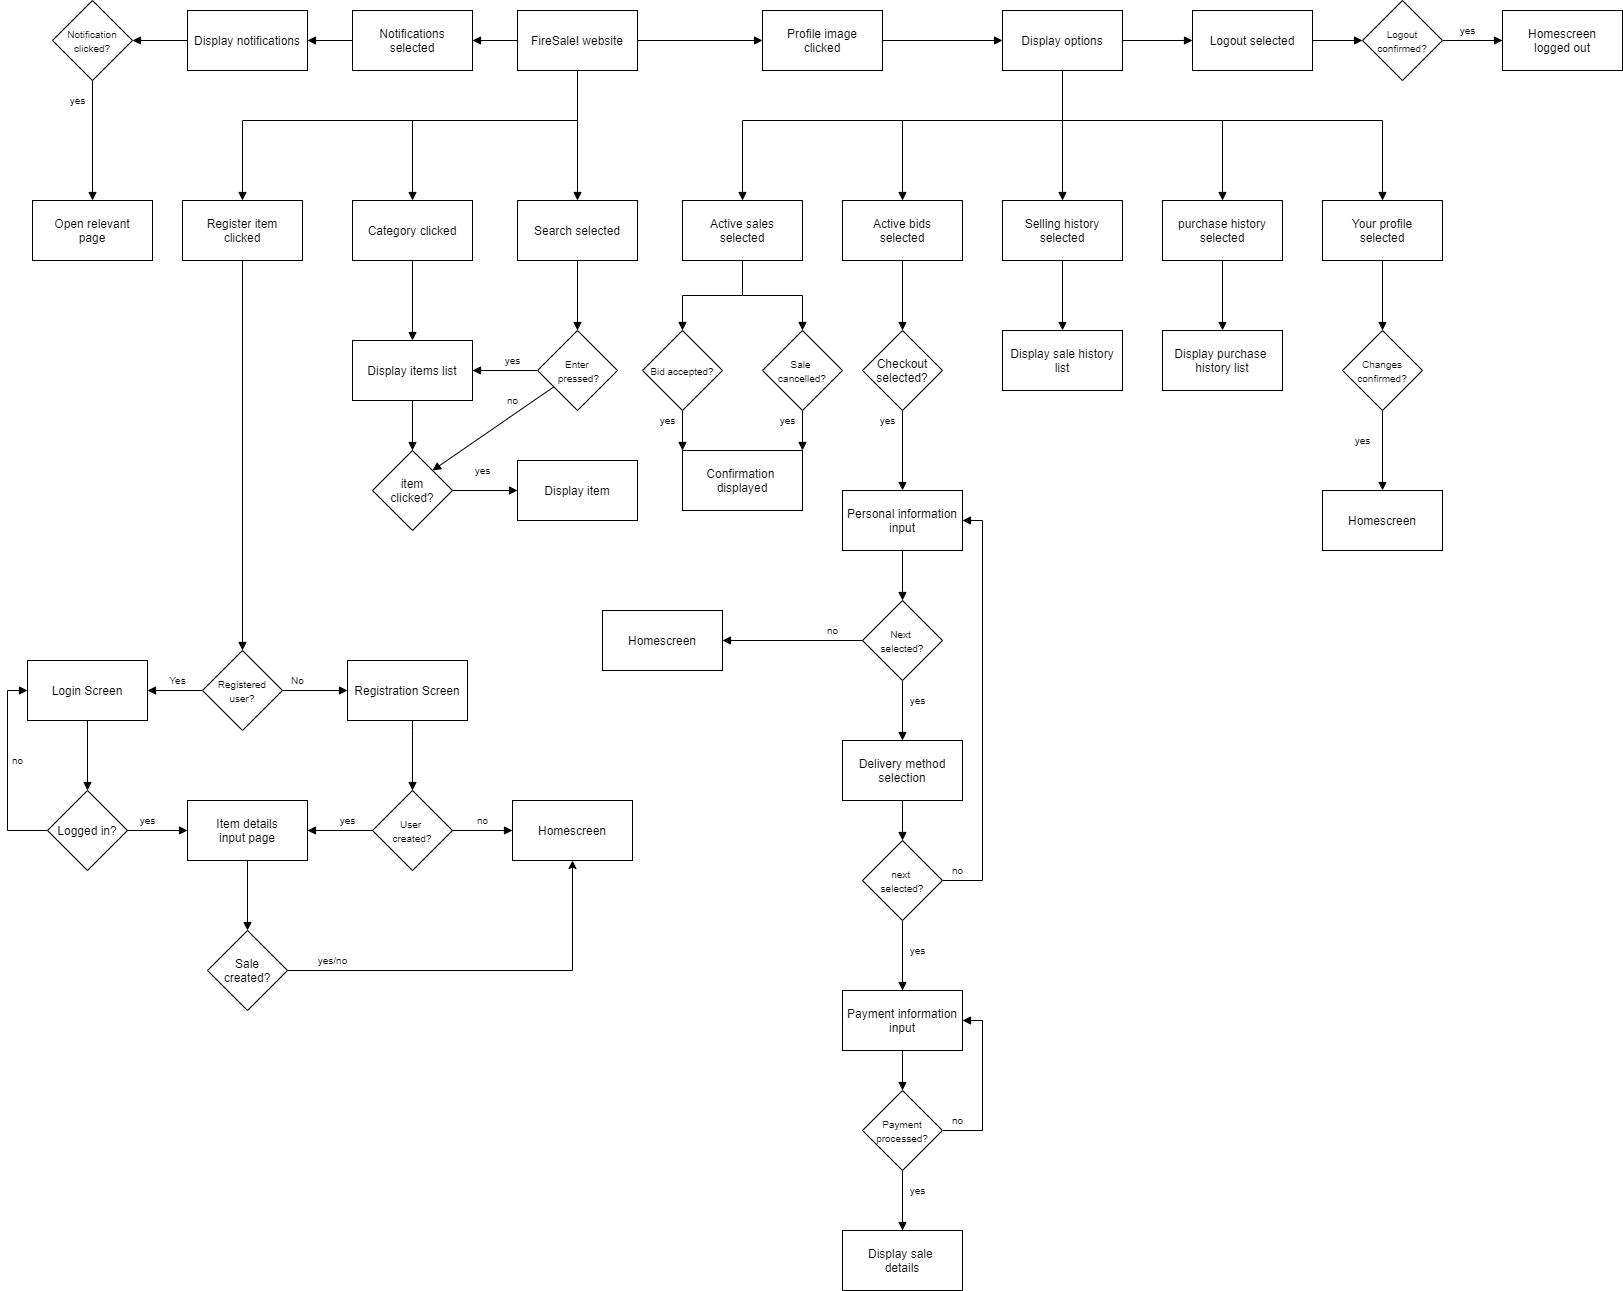
\includegraphics[width=150mm, height=100mm]{Images/NavigationDiagram/NavDiagram.png}\\
\href{https://tinyurl.com/NavigationDiagram}{\textcolor{blue}{Link to the full size navigation diagram.}}
\\\\

\section{Flowchart}

The team created flowcharts to display the process of accepting a bid, how to bid on an item, finish the checkout process of purchasing an item and put an item up for sale. 
\begin{center}
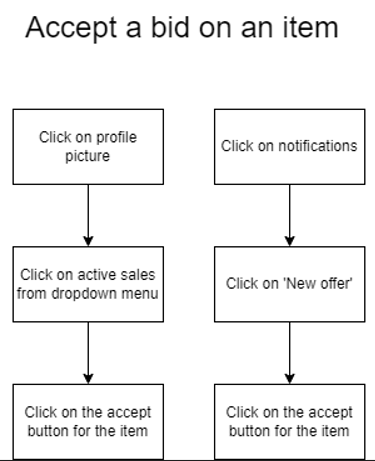
\includegraphics[width=100mm, height=100mm]{Images/FlowChart/accept_a_bid_on_an_item.png}\\[1cm]
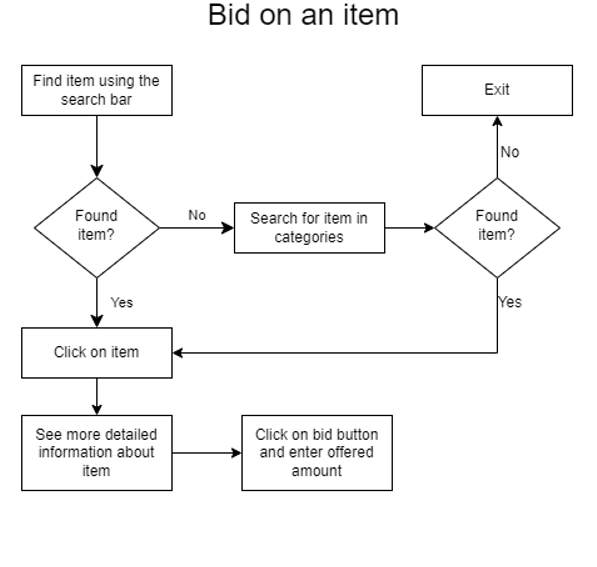
\includegraphics[width=100mm, height=100mm]{Images/FlowChart/Bid_on_an_item.png}
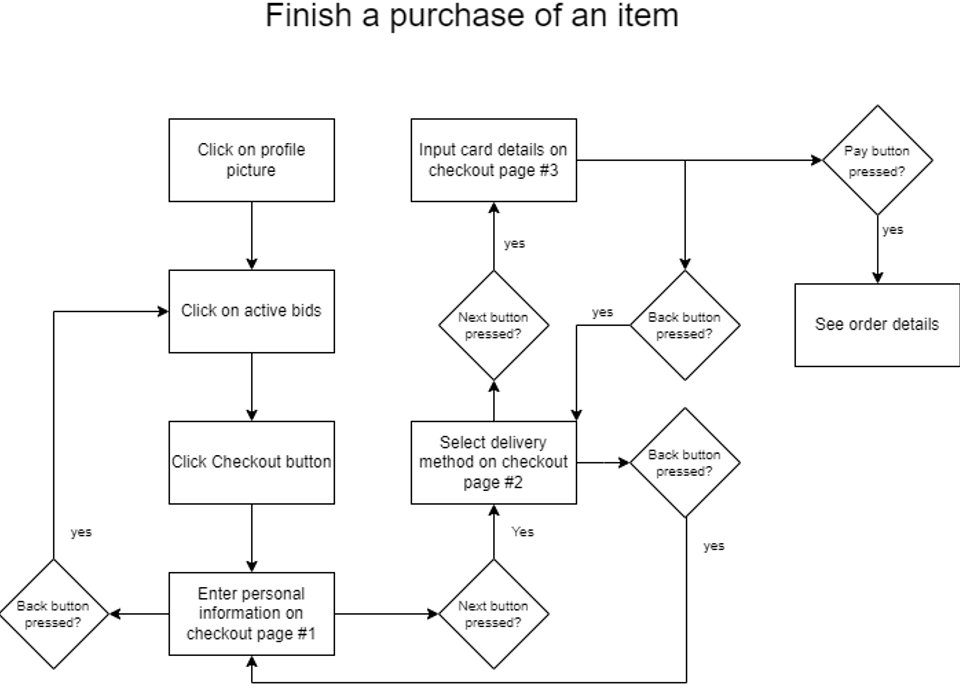
\includegraphics[width=100mm, height=100mm]{Images/FlowChart/finish_a_purchase_of_an_item.png}\\[1cm]
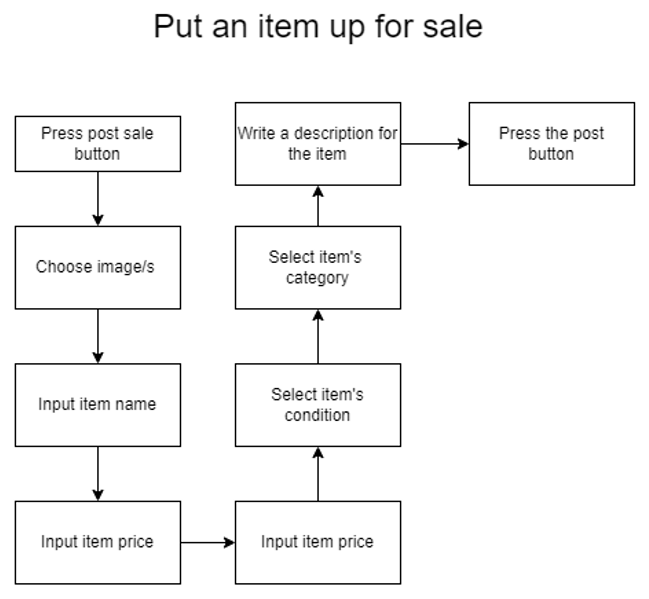
\includegraphics[width=100mm, height=100mm]{Images/FlowChart/put_an_item_up_for_sale.png}
\end{center}

\section{Programming Rules}

In this section we describe code conventions, tooling and coding workflow we intend to use for FireSale!. To start off this section uses \href{https://datatracker.ietf.org/doc/html/rfc2119}{RFC 2119} 
terms when using the phrases: \textit{must}, \textit{must not}, \textit{required}, \textit{shall}, \textit{shall not}, \textit{should}, \textit{should not}, \textit{recommended}, \textit{may}, \& \textit{optional}.\\
 
For version control we are using git, hosting the repo on GitHub, the repos \textit{main} branch is write protected to ensure proper workflow through Pull Requests (PRs). We also utilise \textit{.gitignore} to keep unwanted file out of the repo.\\

To help us keep the code-bases' indents, newlines and encoding consistent across the multiple filetypes and operating systems we use \href{https://editorconfig.org}{\textit{editorconfig}}.\\

The UTF-8 encoding and UNIX newlines are used for all files unless otherwise specified.\\

All PRs merged with the main branch will be linted for code consistency, this is done either manually or with CI if we find time to set it up.

\subsection{Comments}
Through out the code we should comment all functions and classes with some form of docstrings containing a description of what the function does along with listing of parameters and expected output.\\

Inline comments must have two full spaces before and one after the comment symbol/s followed by a short and concise comment.\\

If someone ever notices a bug but for what ever reason can´t deal with at that time it's recommended to comment 'FIXME: <short description or link to Asana>'. For functionality yet to be implemented one should comment 'TODO: <short description or link to Asana>', this makes searching for found bugs and missing functionality easier.\\

\subsection{Directory Structure}

\dirtree{%
    .1 FireSale!.
    .2 .github.
    .3 <ci>.
    .2 docs.
    .3 diagrams.
    .4 <plantUML diagrams>.
    .2 FireSale!.
    .3 <django project files>.
    .2 db.
    .3 <src>.
    .2 tests.
    .2 .editorcofnig.
    .2 .gitignore.
    .2 README.md.
}

\subsection{CSS}
Our CSS code conventions are quite straight forward, everything in a block should be lowercase, use four space soft tab for indenting, and leave a single empty line between blocks.

\subsection{HTML}
HTML files we have more points to consider than for CSS.

\begin{itemize}
	\item all tags and attributes must be in lowercase
	\item opened tags need to be closed
	\item no space around = in attribute assignment
	\item attribute values encased in double quotes
	\item images have alt, width and height defined
	\item \textbf{no inline css or js!}
\end{itemize}

\subsection{Java Script}
JavaScript is probably has the wildest style guides out there, but we decided to follow \href{https://google.github.io/styleguide/jsguide.html}{Googles JS style guide} even if it's a long winded read.

\begin{itemize}
	\item braces should be used with all keywords that support them
	\item semicolons are required
	\item when defining variables use const or let
	\item don't mix quoted and unquoted keys
	\item use JSDOC style comments for classes and functions
	\item variables and functions should be named in camelCase
	\item classes should be named in CamelCase
	\item eval evil
\end{itemize}

\subsection{Python}
For Python we plan on following \href{https://peps.python.org/pep-0008/}{PEP8} as closely one finds reasonable.\\

To give a brief summery on PEP8:
\begin{itemize}
    \item variables and functions are named in snake\_case
    \item space between all operators
    \item space after a comma not before e.g. ", "
    \item leave two empty lines between functions and/or classes, but one line between functions in the same class
    \item all functions and classes should have a docstring summarising their inner workings, parameters, and return values
    \item when defining a function use typing where it applies
\end{itemize}

\subsection{SQL}
Despite SQL not having many points in our code style it's probably has the strangest.

\begin{itemize}
    \item keywords in lowercase
    \item indents should create a 'river' down the length of each given query, between keywords and parameters
    \item indent subqueries should be indented based on how far in the subquerie starts
\end{itemize}

\section{Next steps and changes}
\subsection{Ensuring project readiness and work processes}
To ensure our application will be released on time we will attempt to do Test Driven Development or TDD for short. This methodology is a part of the Agile process (and a fundamental part of the Extreme programming (XP) paradigm).
Although our ambitions will not go as far as to adhere strictly to some formal Agile process, we want to use the red-green-refactor paradigm to both practice creating unit tests and hopefully keep our codebase as bug free as possible.\\

Another process we will be utilizing from the Agile process is daily standup meetings. These meetings should be an outlier for what each team member is working on for the day, if there are any blockers or issues for the tasks and if any team members requires assistance from the rest of the group. \\

The group will be using Asana to keep track of tasks and the project status.\\

We have split the initial responsibility into 3 main categories. Models and the data layer, Services and business logic layer, and finally the views and user facing layer. Our group decided that one member is responsible for the work done inside these layers and the fourth members is responsible for integration of the layers and the overall application cohesion. \\

\subsection{Work hours expectations}
As this course is mimicking a real world team of programmers inside some company, we set our working hours to be 08:00 - 16:00 and attendance to RU is highly encouraged but as a diverse team with varying responsibilities in our private lives these working hours are very flexible.\\

\subsection{Changes}
There is some functionality we had a hard time getting fitting into our prototype. Our idea for how buyer and sellers set up hand-off at some neutral location based on geographic data. The idea was the seller sets up a radius that we could display on a map and the buyer could pick any location there to meet with the buyer.\\

After our user testing, we became aware of some features that would likely benefit our application. One user asked about where the money goes after they accepted a bid and an idea of adding a virtual wallet to our site emerged. This would be a feature that we could add after our basic functionality is met.


\section{Conclusion}

We are a pretty \textbf{soild} team!

\end{document}